\documentclass[11pt]{article}
\usepackage[margin=1in]{geometry}
\usepackage{amsmath,amssymb,amsthm}
\usepackage{graphicx}
\usepackage{microtype}
\usepackage[hidelinks]{hyperref}

\newtheorem{theorem}{Theorem}
\newtheorem{lemma}{Lemma}
\newtheorem{remark}{Remark}
\newcommand{\Aone}{A_1(\mathcal D)}
\newcommand{\Mcal}{\mathcal M}

\title{A weakness spike obstructs the nonmonotone rate formula\\
\large A scoped counterexample for arXiv:2604.26064}
\author{Automated discovery run \texttt{fa\_banach\_001}, lane 6}
\date{August 27, 2026}

\begin{document}
\maketitle

\begin{center}
\fbox{\parbox{0.91\textwidth}{\textbf{Status.}
Candidate scoped counterexample, likely valid, pending expert review.
The result proves that the monotonicity hypothesis in Theorem 1.1 of the
source cannot simply be deleted while retaining its displayed rate and its
dependence on the current weakness parameter. It does not rule out a
different estimate for arbitrary weakness sequences.}}
\end{center}

\section{Source statement and question}

Spivak and Temlyakov study the Weak Greedy Algorithm in a Hilbert space with
a dictionary $\mathcal D$ of unit vectors and weakness sequence
$\tau=(t_k)_{k\geq1}$ \cite{source}. Their Theorem 1.1 states, for a
nonincreasing weakness sequence, that
\begin{equation}\label{source-bound}
 \|f-G_m^\tau(f,\mathcal D)\|
 \leq \left(1+\sum_{k=1}^m t_k^2\right)^{-\alpha/2}
 \|f\|^{1-\alpha}\|f\|_{\Aone}^{\alpha},
 \qquad \alpha\leq\frac{t_m}{t_m+2}.
\end{equation}
The authors explicitly say that they do not know how to remove the
monotonicity assumption.

\begin{figure}[ht]
  \centering
  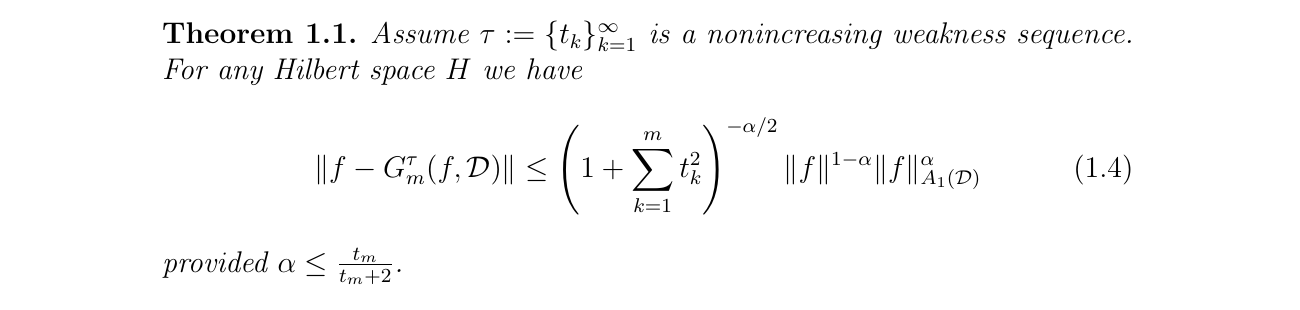
\includegraphics[width=0.95\textwidth]{figures/theorem_1_1_crop.png}
  \caption{The source rate theorem on printed page 3.}
\end{figure}

The following result shows that the literal extension of
\eqref{source-bound} to arbitrary weakness sequences is false, even if a
universal multiplicative constant is allowed.

\section{Statement}

For a residual $r$ define its maximal dictionary correlation by
\[
 \Mcal(r):=\sup_{g\in\mathcal D}|\langle r,g\rangle|.
\]
Recall that one WGA step with weakness $t$ chooses a unit vector
$\varphi\in\mathcal D$ satisfying
$|\langle r,\varphi\rangle|\geq t\Mcal(r)$ and replaces $r$ by
$r-\langle r,\varphi\rangle\varphi$.

\begin{theorem}[One-spike obstruction]\label{main}
There is a number $\varepsilon\in(0,1/2)$ with the following property.
For every $C>0$ there are a real Hilbert space $H$, a dictionary
$\mathcal D\subset H$, a nonzero $f\in\Aone$, a nonmonotone weakness
sequence $\tau$, an index $m$, and a realization of the WGA such that
$t_m=1/2$ and
\begin{equation}\label{counter-bound}
 \|f-G_m^\tau(f,\mathcal D)\|
 > C\left(1+\sum_{k=1}^m t_k^2\right)^{-1/10}
 \|f\|^{4/5}\|f\|_{\Aone}^{1/5}.
\end{equation}
In fact, $\tau$ can be chosen to equal $\varepsilon$ through step $m-1$
and to have a single upward spike $t_m=1/2$ at the tested step.
Consequently, Theorem 1.1 does not remain true after merely deleting
``nonincreasing,'' even up to a universal constant.
\end{theorem}

The exponent $1/10$ in \eqref{counter-bound} is exactly $\alpha/2$ from the
source formula when $t_m=1/2$, since then
$\alpha=t_m/(t_m+2)=1/5$.

\section{Two elementary observations}

The input is the lower-bound theorem quoted as Theorem 5.5 near the end of
the source paper. It is due to Livshitz and Temlyakov \cite{LT}.

\begin{theorem}[Slow constant-weakness realization]\label{LTthm}
There is an absolute constant $b>0$ such that for every $t>0$ one can find
a dictionary $\mathcal D_t$, an element $f_t\in A_1(\mathcal D_t)$, and a
realization of the constant-$t$ WGA whose residuals $r_n$ satisfy
\begin{equation}\label{LTlower}
 \liminf_{n\to\infty} n^{bt}\|r_n\|>0.
\end{equation}
\end{theorem}

The second observation extracts a subsequence on which one stronger greedy
step is harmless.

\begin{lemma}[Slow decay forces small maximal correlation]\label{smallcorr}
Let $0<t<1$ and let $(r_n)$ be a constant-$t$ WGA realization satisfying a
polynomial lower bound
$\|r_n\|\geq c n^{-\gamma}$ for all sufficiently large $n$. Then
\begin{equation}\label{corrzero}
 \liminf_{n\to\infty}\frac{\Mcal(r_n)}{\|r_n\|}=0.
\end{equation}
\end{lemma}

\begin{proof}
If \eqref{corrzero} failed, there would be $\delta>0$ and $n_0$ such that
$\Mcal(r_n)\geq\delta\|r_n\|$ for all $n\geq n_0$. The atom selected at
step $n+1$ would then have correlation at least
$t\delta\|r_n\|$. Since that atom has norm one, the WGA update gives the
exact identity
\[
 \|r_{n+1}\|^2
 =\|r_n\|^2-|\langle r_n,\varphi_{n+1}\rangle|^2
 \leq(1-t^2\delta^2)\|r_n\|^2.
\]
Thus $\|r_n\|$ would decay exponentially, contradicting the assumed
polynomial lower bound.
\end{proof}

\section{Proof of Theorem \ref{main}}

Let $b$ be the absolute constant in Theorem \ref{LTthm}, and fix
\[
 0<\varepsilon<\min\left\{\frac14,\frac{1}{10b}\right\}.
\]
Apply Theorem \ref{LTthm} with $t=\varepsilon$. We obtain fixed
$H,\mathcal D,f$ and a constant-$\varepsilon$ realization with residuals
$r_n$ such that, for some $c>0$ and all sufficiently large $n$,
\begin{equation}\label{poly}
 \|r_n\|\geq c n^{-b\varepsilon}.
\end{equation}
By Lemma \ref{smallcorr}, there is a sequence $N_j\to\infty$ such that
\begin{equation}\label{eta}
 \eta_j:=\frac{\Mcal(r_{N_j})}{\|r_{N_j}\|}\longrightarrow0.
\end{equation}

For a chosen $N=N_j$, define an infinite weakness sequence by
\[
 t_k=\varepsilon\quad(1\leq k\leq N),
 \qquad t_{N+1}=\frac12,
 \qquad t_k=\varepsilon\quad(k\geq N+2).
\]
Use the fixed constant-$\varepsilon$ realization through step $N$. At step
$N+1$, choose any atom permitted by weakness $1/2$ and denote the new
residual by $r'_{N+1}$. Such an atom exists by the definition of a supremum.
Irrespective of which permitted atom is chosen, its correlation is at most
$\Mcal(r_N)$, and hence
\begin{equation}\label{spikeharmless}
 \|r'_{N+1}\|^2
 =\|r_N\|^2-|\langle r_N,\varphi_{N+1}\rangle|^2
 \geq(1-\eta_j^2)\|r_N\|^2.
\end{equation}
Combining \eqref{poly}, \eqref{eta}, and \eqref{spikeharmless}, for all
large $j$ we have
\begin{equation}\label{reslower}
 \|r'_{N_j+1}\|\geq \frac c2 N_j^{-b\varepsilon}.
\end{equation}

At the spike index $m=N_j+1$,
\[
 \sum_{k=1}^{m}t_k^2=N_j\varepsilon^2+\frac14.
\]
Therefore the ratio of the left side of \eqref{counter-bound} to its right
side without $C$ is bounded below by a positive fixed constant times
\[
 N_j^{1/10-b\varepsilon}.
\]
The norms of the fixed vector $f$ are independent of $j$, and
$1/10-b\varepsilon>0$ by construction. The ratio tends to infinity. Given
$C$, choose $j$ large enough. This proves \eqref{counter-bound} and the
theorem.

\section{Scope and interpretation}

The obstruction is not a divergence example: the sequence is tested at one
upward spike, and the construction varies the spike location to contradict
any uniform all-sequences estimate of the form \eqref{source-bound}. It says
that a rate exponent cannot be determined from the current value $t_m$ while
the accumulated gain counts all previous $t_k^2$ without also recording the
order of the weaknesses.

The result leaves several possibilities open. A valid arbitrary-sequence
theorem might use the running minimum $\min_{k\leq m}t_k$, a blockwise
regularity statistic, or an order-sensitive functional in place of $t_m$.
It also does not answer the source's broad Problems 1 and 2 concerning exact
convergence criteria for other greedy algorithms.

\begin{thebibliography}{9}
\bibitem{source}
A. S. Spivak and V. N. Temlyakov,
\emph{On weak greedy algorithms}, arXiv:2604.26064 (2026).

\bibitem{LT}
E. D. Livshitz and V. N. Temlyakov,
\emph{Two lower estimates in greedy approximation},
Constr. Approx. \textbf{19} (2003), 509--523.
\end{thebibliography}

\end{document}
